\chapter{Beispiele}

\addtocontents{lof}{\vspace*{.5cm}{\bf 6~~Beispiele\\}}
%\addtocontents{lot}{\vspace*{.5cm}{\bf 6~~Beispiele\\}}


Im Ordner {\tt example} finden sich umfangreichere Beispiele:


%%%%%%%%%%%%%%%%%%%%%%%%%%%%%%%%%%%%%%%%%%%%%%%%%%%%%%%%%%%%%%%%%%%%%%%%%%%%%55

\section{Chemischer Reaktor}

Bei diesem Modell handelt es sich um eine zweistufige Reaktionsgleichung zur Umwandlung einer chemischen Substanz. Der Temperatur im Reaktor kann durch die Steuerung beeinflusst werden, um die Umwandlung zu beg�nstigen. Ziel ist es, die Konzentration der entstehenden Substanz $x_2$ im Endpunkt zu maximieren. 

$$\begin{array}{crclrcll} \displaystyle\min_{x,u} &\multicolumn{3}{l}{-x_2(1)}\\ 
\text{unter} &\dot x_1(t) &=& -u(t)\cdot x_1(t) + u(t)^2\cdot x_2(t) \\
             &\dot x_2(t) &=&  u(t)\cdot x_1(t) -3\cdot u(t)^2\cdot x_2(t) \\[.1cm] 
             &x_1(0) &=& 1 \\ 
             &x_2(0) &=& 0 \\[.1cm] 
             &u(t)&\in&\multicolumn{5}{l}{[0;1],\quad t\in[0;1]}
\end{array}$$

Quelle: 8.16 bzw. Skript?


\begin{figure}[h]
\begin{center}
\begin{tabular}{|c|c|c|}
\hline
Anzahl Punkte & Zielfunktionswert & Rechenzeit\\\hline
21        &  -0.28810463835 & \\\hline
\end{tabular}

\includegraphics[width=5cm]{images/chemie/pix_1_x_1}
\includegraphics[width=5cm]{images/chemie/pix_2_x_2}
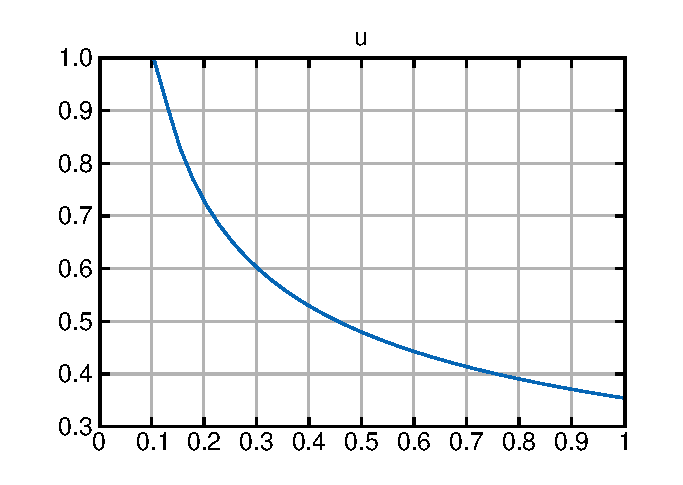
\includegraphics[width=5cm]{images/chemie/pix_3_u}

% \includegraphics[width=5cm]{images/chemie/pix_4_DF}
% 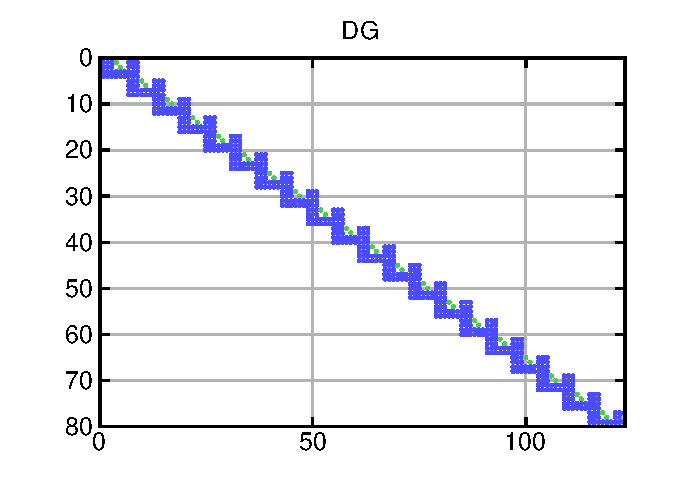
\includegraphics[width=5cm]{images/chemie/pix_5_DG}
% 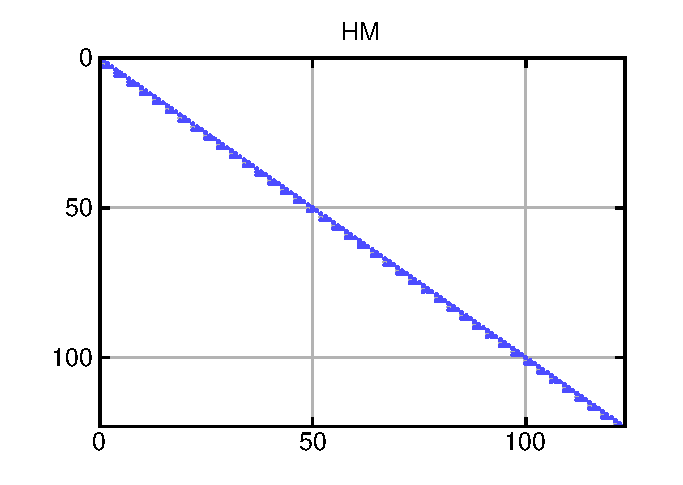
\includegraphics[width=5cm]{images/chemie/pix_6_HM}

\label{ex:chemie}
\caption{Chemischer Reaktor}
\end{center}
\end{figure}


%%%%%%%%%%%%%%%%%%%%%%%%%%%%%%%%%%%%%%%%%%%%%%%%%%%%%%%%%%%%%%%%%%%%%%%%%%%%%55
\newpage
\section{Spline}

Interpolation durch kubischen Spline als Optimierungsaufgabe.

$$\begin{array}{crclrcll} \displaystyle\min_{x,u} &\multicolumn{3}{l}{\frac{1}{2} x_3(1)}\\ 
\text{unter} &\dot x_1(t) &=& x_2(t) \\
             &\dot x_2(t) &=&  u(t) \\
	     &\dot x_3(t) &=&  u^2(t) \\[.1cm]  
             &x_1(0) &=& 0 &  &x_1(1) &=& 0 \\
             &x_2(0) &=& 1  & &x_2(1) &=& -1\\
	     &x_3(0) &=& 0 \\[.1cm] 
             &x_1(t)&\le&\multicolumn{5}{l}{\alpha,\quad t\in[0;1]}
\end{array}$$

$\alpha > 1/4$: unbeschr�nkt

$1/6<\alpha<1/4$: Ber�hrpunkt

$1/6>\alpha$: Randst�ck



\begin{tabular}{ll}
Diskretisierung & 21 Punkte\\
Zielfunktionswert $\alpha=0$ & 1.9999986332\\
Zielfunktionswert $\alpha=\frac{1}{6}$ &  2.6666658193
\end{tabular}

Quelle: 10.14 bzw. Skript?



\begin{figure}[h]
\begin{center}
\includegraphics[width=5cm]{images/spline/pix_1_x_1}
\includegraphics[width=5cm]{images/spline/pix_2_x_2}
\includegraphics[width=5cm]{images/spline/pix_3_x_3}
\includegraphics[width=5cm]{images/spline/pix_4_u}

% 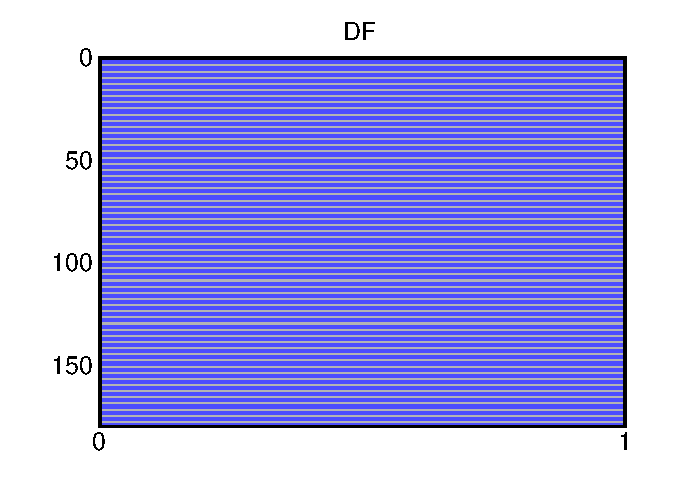
\includegraphics[width=5cm]{images/spline/pix_5_DF}
% 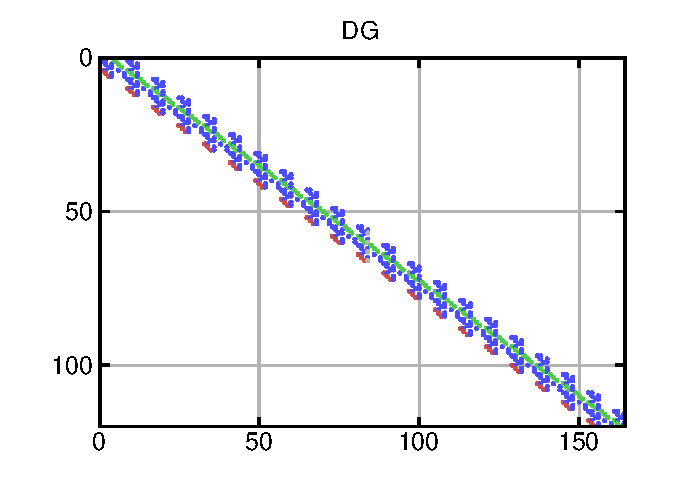
\includegraphics[width=5cm]{images/spline/pix_6_DG}
% 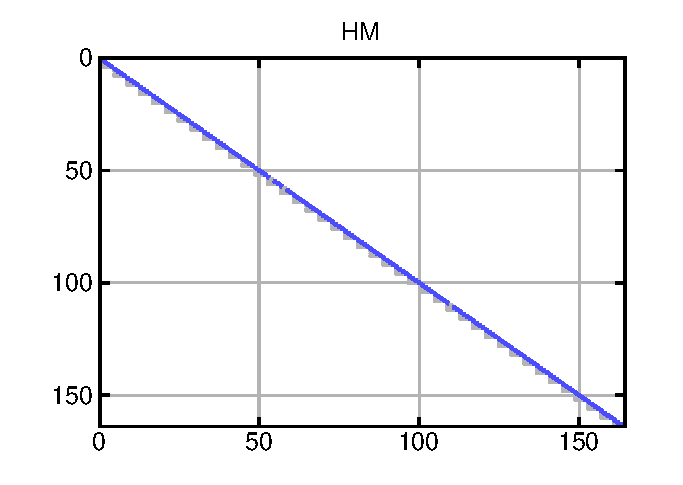
\includegraphics[width=5cm]{images/spline/pix_7_HM}

\label{ex:spline}
\caption{L�sung Spline-Problem mit $\alpha=\frac{1}{6}$}
\end{center}
\end{figure}


\explain{Das Programm zeigt, wie sich Parameter �ber die Kommandozeile variieren lassen.
Hierzu wird eine map der Kommandozeilenparameter ausgelesen.

Die Beschr�nkung $\alpha$ l�sst sich �ber --c steuern.
}

\verb+spline -n 21 --c 0.166666+









%%%%%%%%%%%%%%%%%%%%%%%%%%%%%%%%%%%%%%%%%%%%%%%%%%%%%%%%%%%%%%%%%%%%%%%%%%%%%55
\newpage
\section{Unged�mpfter harmonischer Oszillator}
Beispiel mit freier Endzeit. Die freie Endzeit wird in $p_0$ abgelegt. Das DGl-System muss mit $p_0$ multipliziert werden.


$$\begin{array}{crclrcll} \displaystyle\min_{x,u,t_f} &\multicolumn{3}{l}{t_f}\\ 
\text{unter} &\dot x_1(t) &=& x_2(t) \\
             &\dot x_2(t) &=& -x_1(t)+u(t) \\[.1cm]    
             &x(0)        &=& \left(\begin{array}{c}3\\1\end{array}\right) 
             &x(t_f)      &=& \left(\begin{array}{c}0\\0\end{array}\right) \\[.1cm] 
             &u(t)&\in&[-1;1],& t\in[0;t_f]
\end{array}$$


\begin{tabular}{ll}
Diskretisierung & 51 Punkte\\
Zielfunktionswert & 5.2160656622\\
\end{tabular}

Quelle: 5.19


\begin{figure}[h]
\begin{center}
\includegraphics[width=5cm]{images/oszillator/pix_1_x_1}
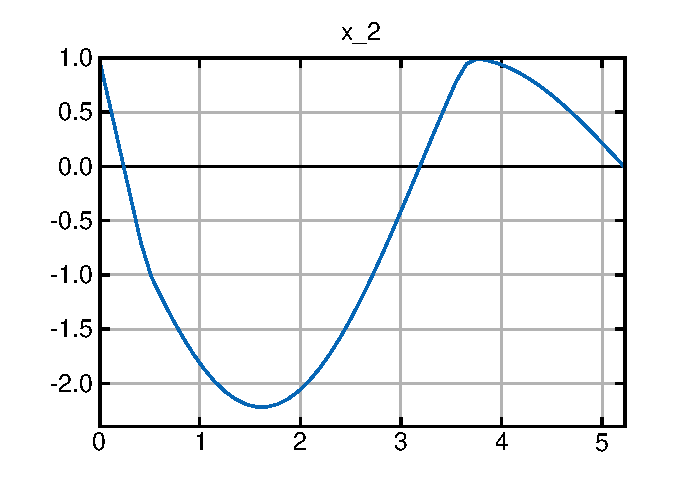
\includegraphics[width=5cm]{images/oszillator/pix_2_x_2}
\includegraphics[width=5cm]{images/oszillator/pix_3_u}

\label{ex:oszillator}
\caption{L�sung Oszillator-Problem}
\end{center}
\end{figure}

\explain{
{\tt freetime = 1;} stellt freie Endzeit auch im Viewer dar.
}




\newpage
\section{Raketenwagen}

Gasgeben und Bremsen.



$$\begin{array}{crclrcll} \displaystyle\min_{x,u,t_f} &\multicolumn{3}{l}{t_f}\\ 
\text{unter} &\dot x_1(t) &=& x_2(t) \\
             &\dot x_2(t) &=& u(t) \\[.1cm]    
             &x(0)        &=& \left(\begin{array}{c}4\\-1\end{array}\right) 
             &x(t_f)      &=& \left(\begin{array}{c}0\\0\end{array}\right) \\[.1cm] 
             &u(t)&\in&[-1;1],& t\in[0;t_f]
\end{array}$$


\begin{tabular}{ll}
%Diskretisierung & 51 Punkte\\
%Zielfunktionswert & 5.2160656622\\
\end{tabular}

Quelle: ?


\begin{figure}[h]
\begin{center}
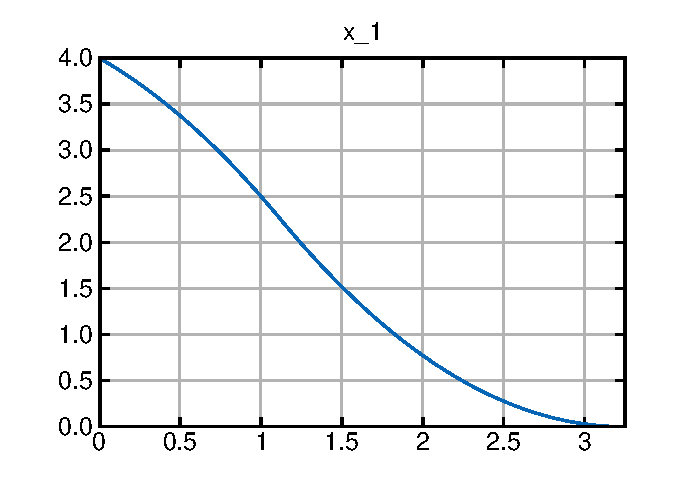
\includegraphics[width=5cm]{images/rakete/pix_1_x_1}
\includegraphics[width=5cm]{images/rakete/pix_2_x_2}
\includegraphics[width=5cm]{images/rakete/pix_3_u}

\label{ex:rakete}
\caption{L�sung Raketenwagen-Problem}
\end{center}
\end{figure}







%%%%%%%%%%%%%%%%%%%%%%%%%%%%%%%%%%%%%%%%%%%%%%%%%%%%%%%%%%%%%%%%%%%%%%%%%%%%%55
\newpage
\section{Erzentlader}

$$\begin{array}{crclrcll} \displaystyle\min_{x,u,t_f} &\multicolumn{3}{l}{t_f}\\ 
\text{unter} &\dot x_1(t) &=& x_2(t) \\
             &\dot x_2(t) &=&  u(t) \\
	     &\dot x_3(t) &=&  x_4(t) \\
	      &\dot x_4(t) &=&  -x_3(t)+u(t) \\[.1cm]    
       &x(0) &=& \left(\begin{array}{c}0\\0\\0\\0\end{array}\right) 
&x(t_f) &=& \left(\begin{array}{c}1\\0\\0\\0\end{array}\right) \\[.1cm] 
             &u(t)&\in&[-1;1],& t\in[0;t_f]\\
	    &x_2(t)&\le&0.2,& t\in[0;t_f]
\end{array}$$





\begin{tabular}{ll}
Diskretisierung & 101 Punkte\\
Zielfunktionswert & 5.84412332892\\
\end{tabular}

Quelle: 10.11


\begin{figure}[h]
\begin{center}
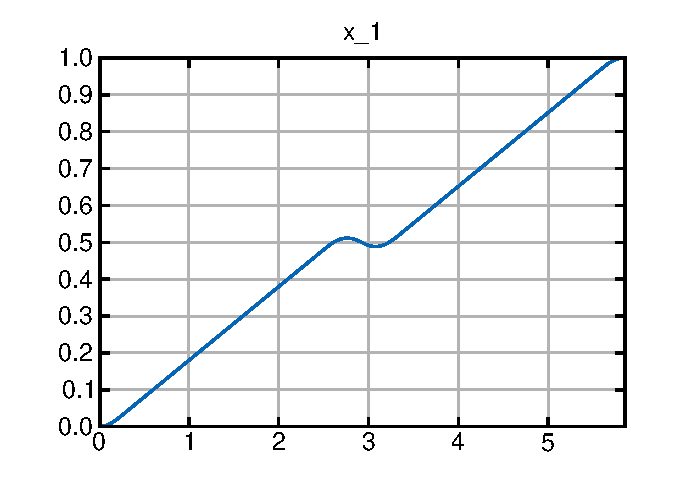
\includegraphics[width=5cm]{images/erzentlader/pix_1_x_1}
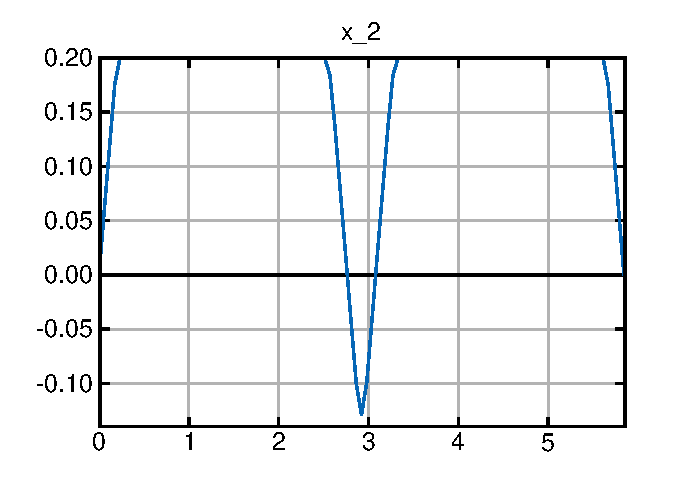
\includegraphics[width=5cm]{images/erzentlader/pix_2_x_2}
\includegraphics[width=5cm]{images/erzentlader/pix_3_x_3}
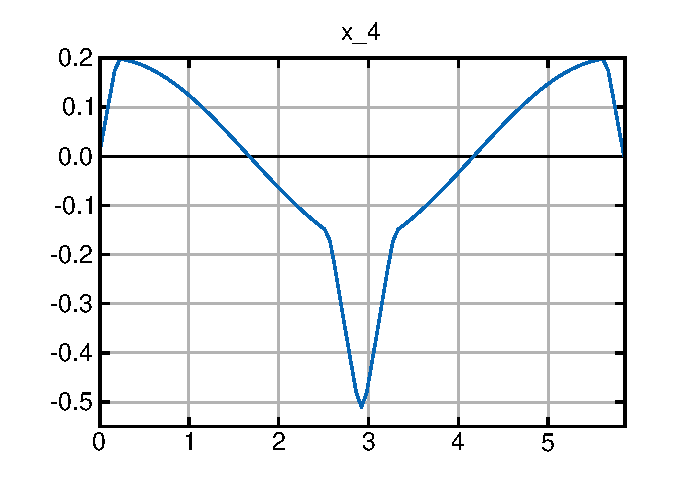
\includegraphics[width=5cm]{images/erzentlader/pix_4_x_4}
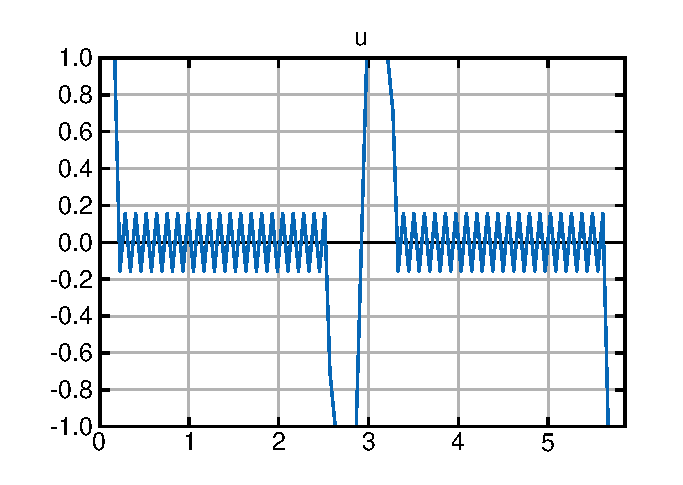
\includegraphics[width=5cm]{images/erzentlader/pix_5_u}


\label{ex:erzentlader}
\caption{L�sung Erzentlader}
\end{center}
\end{figure}






%%%%%%%%%%%%%%%%%%%%%%%%%%%%%%%%%%%%%%%%%%%%%%%%%%%%%%%%%%%%%%%%%%%%%%%%%%%%%55
\newpage
\section{Knickstab}

$$\begin{array}{crclrcll} \displaystyle\min_{x,u} &\multicolumn{3}{l}{\displaystyle\int\limits_0^1 \frac{1}{2} u(t)^2 + \alpha\cdot \cos\theta(t) \, dt}\\ 
\text{unter} &\dot x(t) &=& \sin\theta(t) \\
             &\dot \theta(t) &=&  u(t) \\[.1cm]    
       &x(0) &=& 0   & x(1) &=& 0 \\[.1cm] 
             &x(t)&\in&[-0.05;0.05],& t\in[0;1]
\end{array}$$


\explain{
Alternative Formulierungen als {\tt knickstab.cpp} und {\tt knickstab\_int.cpp}
 mit Lagrange-Term
}

\explain{
TolOpti wird intern h�her gesetzt.
}

\begin{tabular}{ll}
Diskretisierung $\alpha=9.90027$ & 60 Punkte\\
Zielfunktionswert & 9.9002014316\\
\end{tabular}

\begin{tabular}{ll}
Diskretisierung $\alpha=27.2627$ & 51 Punkte\\
Zielfunktionswert & 27.151069208\\
\end{tabular}

\begin{tabular}{ll}
Diskretisierung $\alpha=150$ & 180 Punkte\\
Zielfunktionswert & 148.51217659
\end{tabular}

Quelle: ?




\begin{figure}[h]
\begin{center}
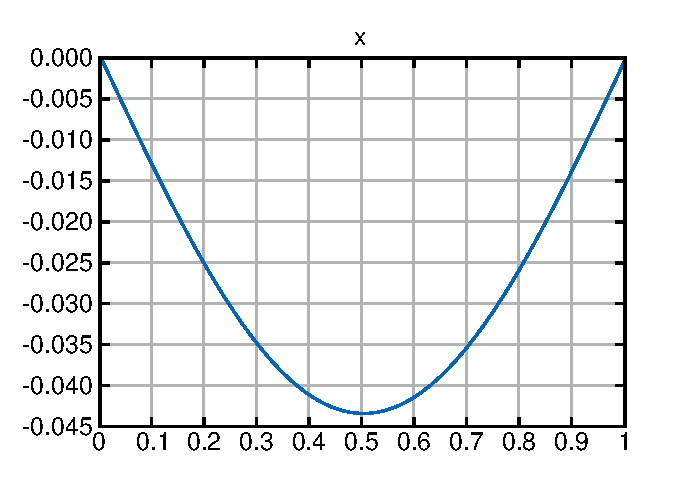
\includegraphics[width=5cm]{images/knickstab_int_9/pix_1_x}
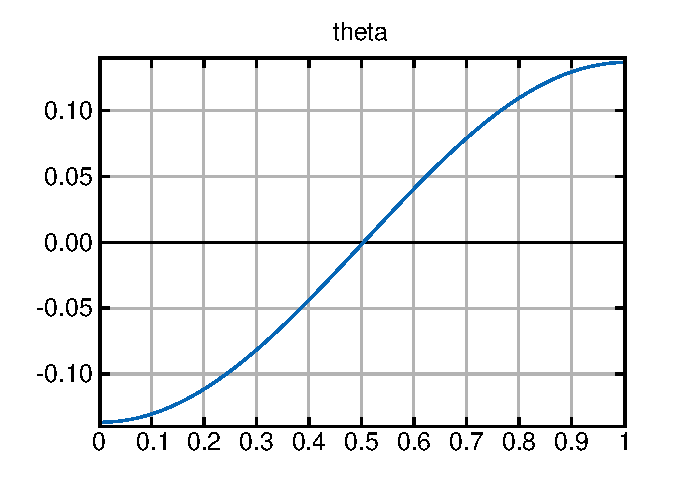
\includegraphics[width=5cm]{images/knickstab_int_9/pix_2_theta}
\includegraphics[width=5cm]{images/knickstab_int_9/pix_3_u}
%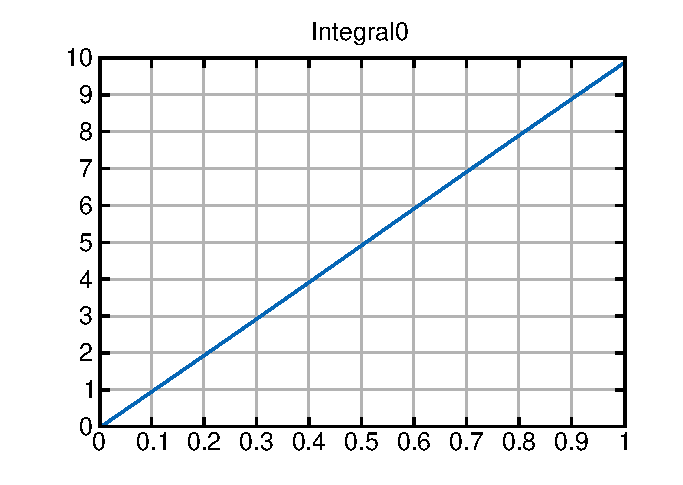
\includegraphics[width=5cm]{images/knickstab_int_9/pix_4_Integral0}

\label{ex:knick1}
\caption{L�sung Knickstab f�r $\alpha=9.90027$}
\end{center}
\end{figure}



\begin{figure}[h]
\begin{center}
\includegraphics[width=5cm]{images/knickstab_int_27/pix_1_x}
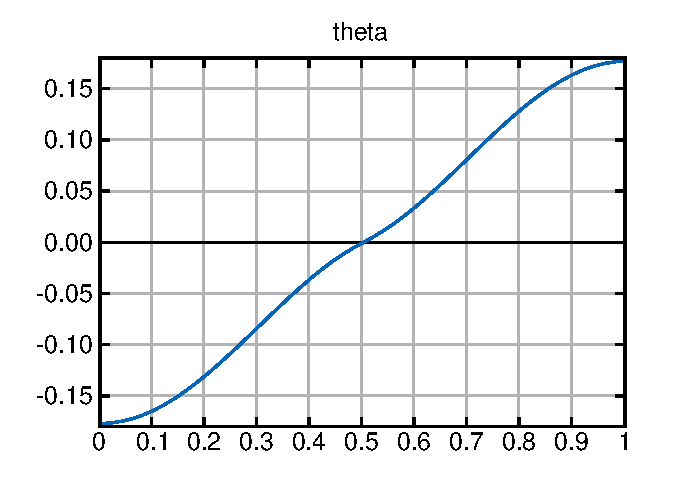
\includegraphics[width=5cm]{images/knickstab_int_27/pix_2_theta}
\includegraphics[width=5cm]{images/knickstab_int_27/pix_3_u}
%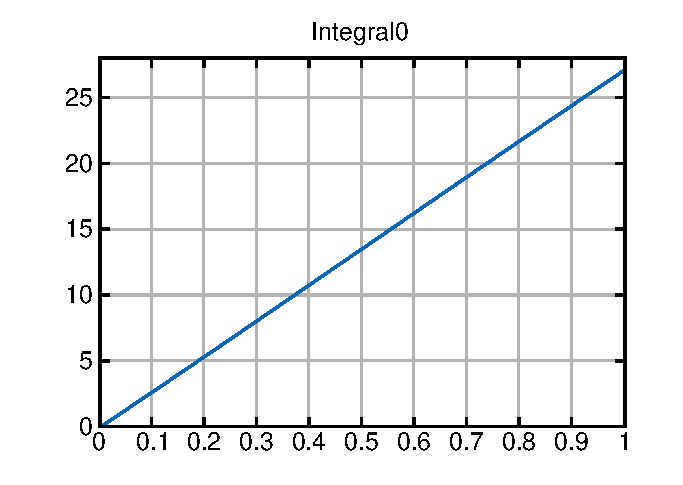
\includegraphics[width=5cm]{images/knickstab_int_27/pix_4_Integral0}

\label{ex:knick2}
\caption{L�sung Knickstab f�r $\alpha=27.2627$}
\end{center}
\end{figure}


\begin{figure}[h]
\begin{center}
\includegraphics[width=5cm]{images/knickstab_int_150/pix_1_x}
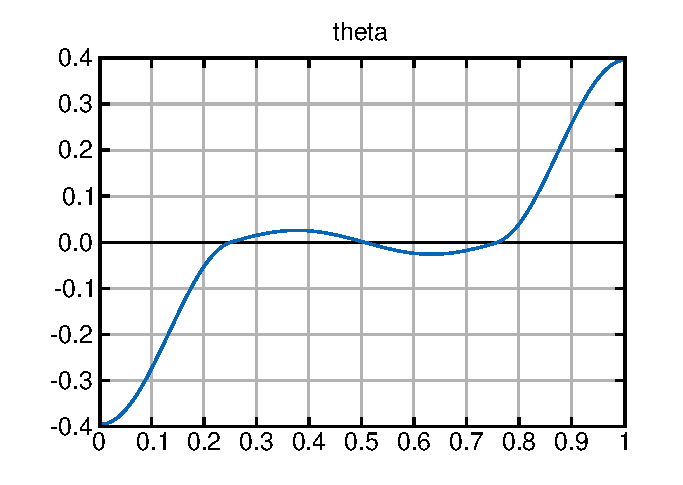
\includegraphics[width=5cm]{images/knickstab_int_150/pix_2_theta}
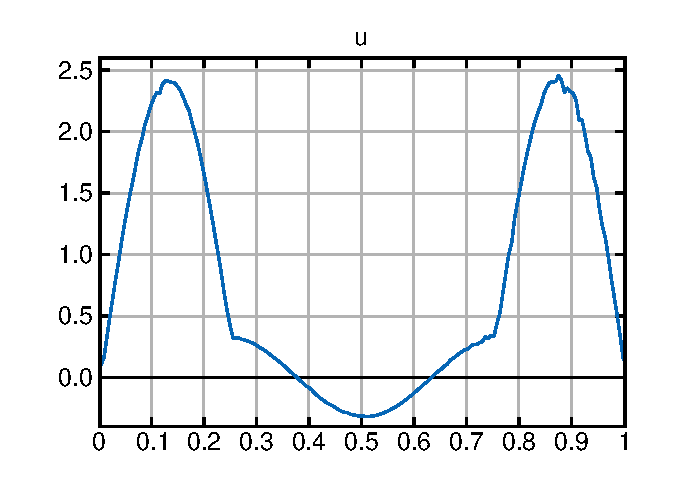
\includegraphics[width=5cm]{images/knickstab_int_150/pix_3_u}
%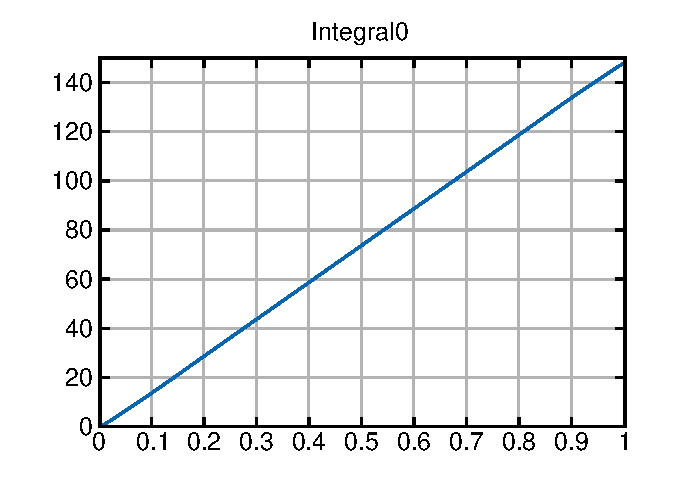
\includegraphics[width=5cm]{images/knickstab_int_150/pix_4_Integral0}

\label{ex:knick3}
\caption{L�sung Knickstab f�r $\alpha=150$}
\end{center}
\end{figure}






%%%%%%%%%%%%%%%%%%%%%%%%%%%%%%%%%%%%%%%%%%%%%%%%%%%%%%%%%%%%%%%%%%%%%%%%%%%%%55
\newpage
\section{Reentry-Problem}

$$\begin{array}{crclrcll} \displaystyle\min_{} &\multicolumn{3}{l}{\displaystyle\int\limits_0^{t_f} 10 v^3\sqrt{p_0 e^{-\beta R xi}}}\\ 
\text{unter} &\dot v &=& -\frac{S p v^2}{2m} C_W(u) - \frac{g \sin\gamma}{(1+\xi)^2} \\
  &\dot \gamma &=& -\frac{S p v}{2m} C_A(u) + \frac{v \cos\gamma}{R (1+\xi)} 
- \frac{g \sin\gamma}{v\cdot(1+\xi)^2}\\
             &\dot \xi(t) &=&  \frac{v \sin\gamma}{R} 	      \\[.1cm]    
   \text{mit}  &p &=& p_0 e^{-\beta R\xi}\\
&C_W(u) &=& 1.174 - 0.9\cos u \\
&C_A(u) &=& 0.6\sin u \\[.1cm]
&v(0) &=& 0.36 & v(t_f) &=& 0.27 \\
&\gamma(0) &=& -8.1 \cdot \frac{\pi}{180} & \gamma(t_f) &=& 0 \\
&\xi(0) &=& \frac{4}{R} & \xi(t_f) &=& \frac{2.5}{R}             
\end{array}$$

$$R = 209, \beta = 4.26, p_0 = 2.704\cdot 10^{-3}, g = 3.2172\cdot 10^{-4}, \frac{S}{m} = 53200 $$




\begin{tabular}{ll}
Diskretisierung & 71 Punkte\\
Zielfunktionswert & 0.027911689692\\
Final Time & 225.427        
\end{tabular}

Quelle: ?


\begin{figure}[h]
\begin{center}
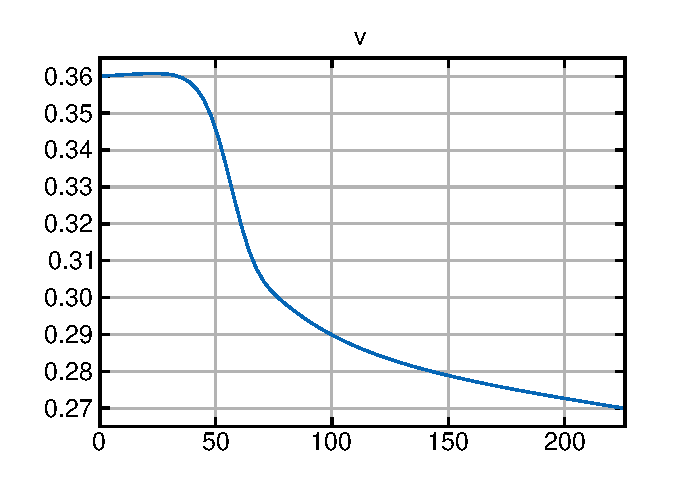
\includegraphics[width=5cm]{images/reentry/pix_1_v}
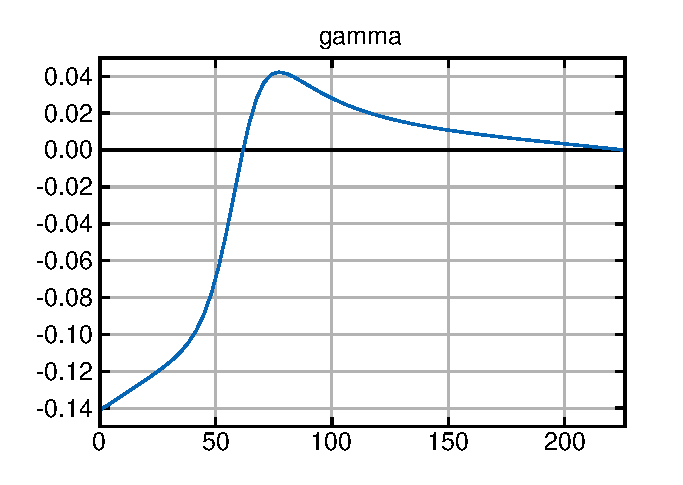
\includegraphics[width=5cm]{images/reentry/pix_2_gamma}
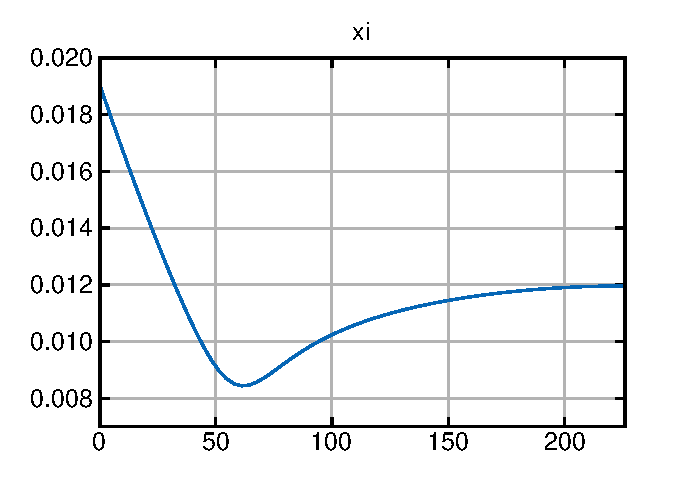
\includegraphics[width=5cm]{images/reentry/pix_3_xi}
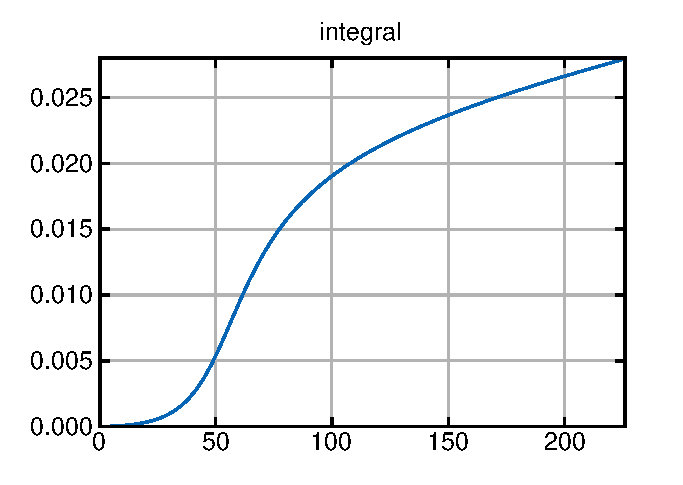
\includegraphics[width=5cm]{images/reentry/pix_4_integral}
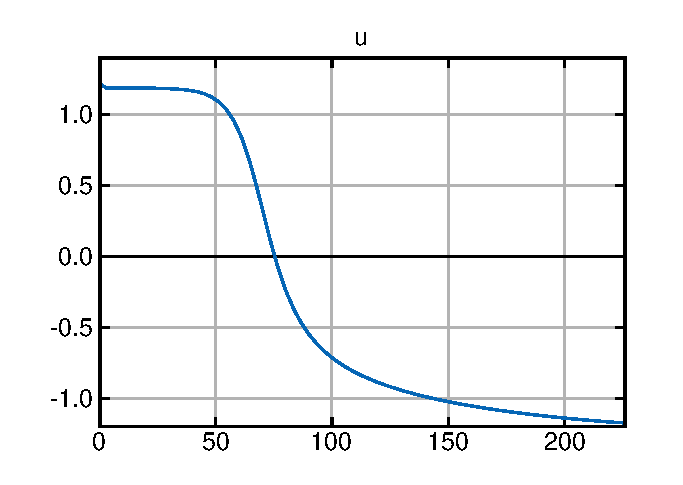
\includegraphics[width=5cm]{images/reentry/pix_5_u}


\label{ex:reentry}
\caption{L�sung Reentry-Problem}
\end{center}
\end{figure}

\explain{Funktion terminate zur Ausgabe der Verfahrzeit nach Optimierung}

\explain{Funktion step zur Manipulation der L�sung (hier abschneiden auf $[-\pi,\pi]$)}

\explain{alternative formulierung mit sin/cos und Nebenbedingung}



%%%%%%%%%%%%%%%%%%%%%%%%%%%%%%%%%%%%%%%%%%%%%%%%%%%%%%%%%%%%%%%%%%%%%%%%%%%%%55

\newpage
\section{Laufkatze}

Kransystem

\begin{figure}
\begin{center}
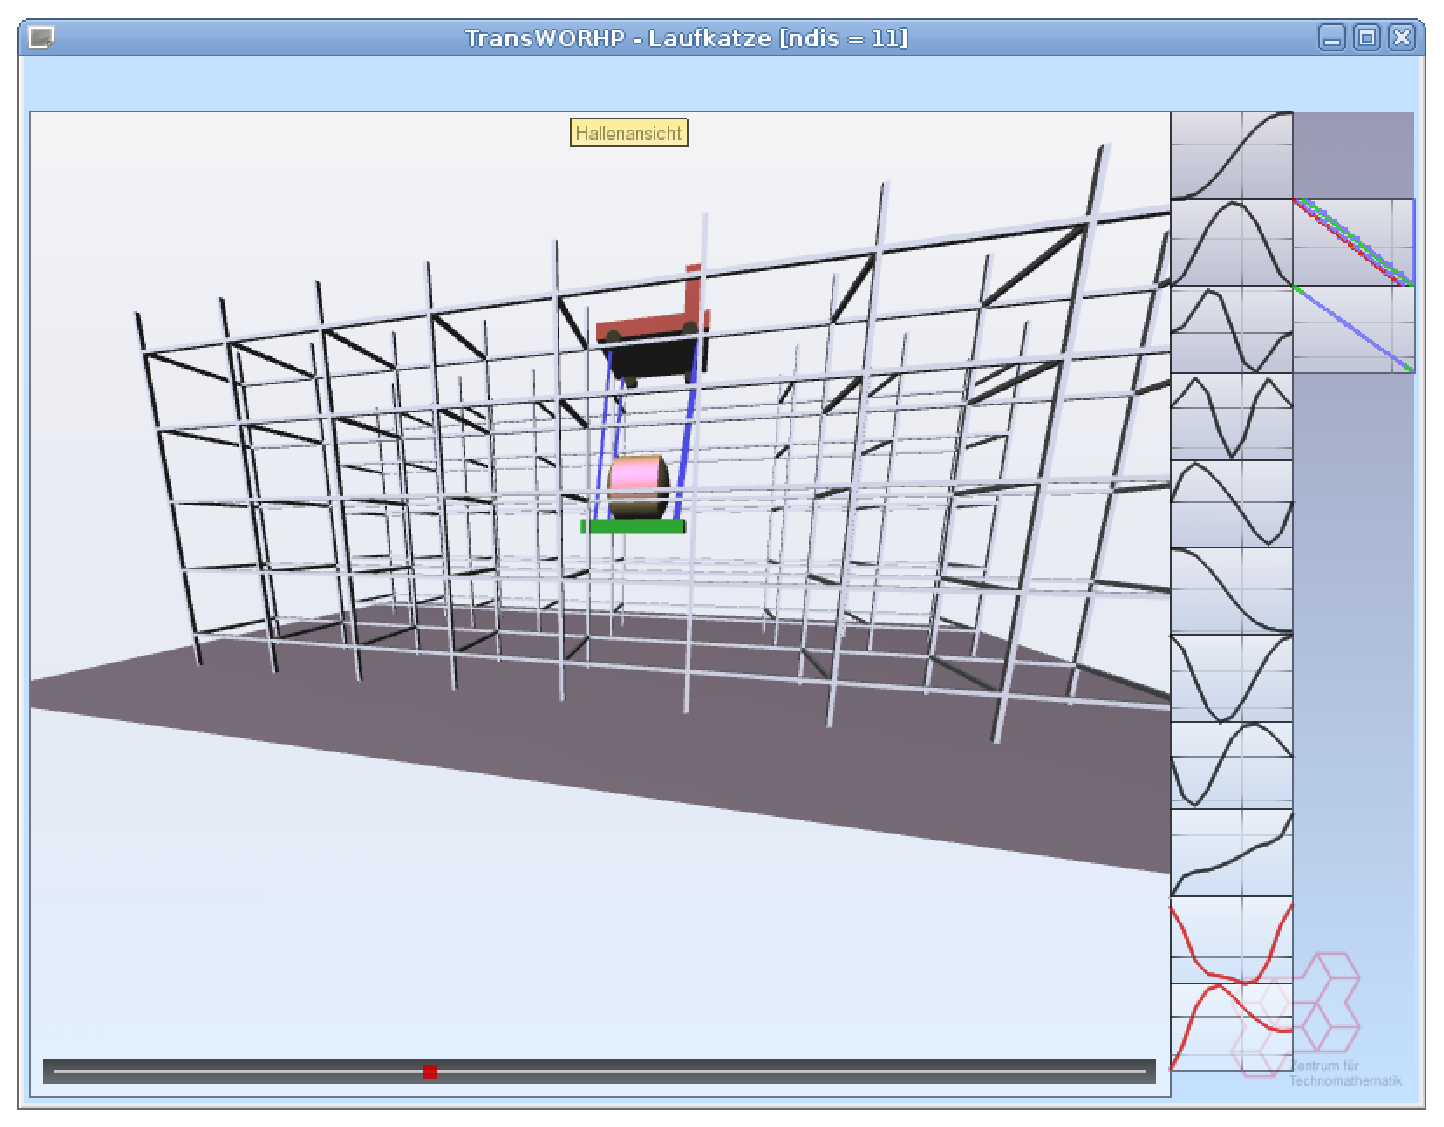
\includegraphics[width=10cm]{images/laufkatze}
\caption{3d-Plot der Laufkatze}
\label{abb3}
\end{center}
\end{figure}

\begin{itemize}
\item Standardproblem
\item mit Automatischer Differentiation
\item in Lagrange-Formulierung
\end{itemize}

\begin{align*} \label{eq:laufkateze}
\begin{split}
	\min_{x,u,t_f} \qquad & x_8(t_f) + 0.1 \cdot t_f\\
	\text{unter} \quad \dot{x}_0 &= x_1 \cdot t_f\\
	\dot{x}_1 &= x_4 \cdot t_f\\
	\dot{x}_2 &= x_3 \cdot t_f\\
	\dot{x}_3 &= \left(x_4 - (9.81-x_7)\cdot \frac{x_2}{x_5}\right)  \cdot t_f\\
	\dot{x}_4 &= u_0 \cdot t_f\\
	\dot{x}_5 &= x_6 \cdot t_f\\
	\dot{x}_6 &= x_7 \cdot t_f\\
	\dot{x}_7 &= u_1 \cdot t_f\\
	\dot{x}_8 &= \left(u_0^2 + u_1^2\right) \cdot t_f\\
	x(0) &= (0,0,0,0,0,5,0,0,0)^\top\\
	x(t_f) &= (8,0,0,0,0,4,0,0,\text{frei})^\top\\
	-1 &\leq u_0(t) \leq 1, -1 \leq u_1(t) \leq 1\\
	0 &\leq x_0(t) \leq 100, -3 \leq x_1(t) \leq 3\\
	-2 &\leq x_2(t) \leq 2, -10 \leq x_3(t) \leq 10\\
	-4 &\leq x_4(t) \leq 4, 0.5 \leq x_5(t) \leq 15\\
	-3 &\leq x_6(t) \leq 3, -10 \leq x_7(t) \leq 10\\
	0 &\leq x_8(t), \text{ f�r alle } t \in [0,t_f]
\end{split}
\end{align*}


%%%%%%%%%%%%%%%%%%%%%%%%%%%%%%%%%%%%%%%%%%%%%%%%%%%%%%%%%%%%%%%%%%%%%%%%%%%%%55

\newpage
\section{Beschr�nkter Spline}
wie im Tutorial, mit einer zus�tzlichen Beschr�nkung

\section{Brachistochrone}
Kurve der schnellsten Fallzeit






\section{Roboter}

Industrie-Roboter mit 3 Freiheitsgraden



\section{Geo-Leo-Transfer}

Raumf�hre fliegt um die Erde.

\begin{figure}
\begin{center}
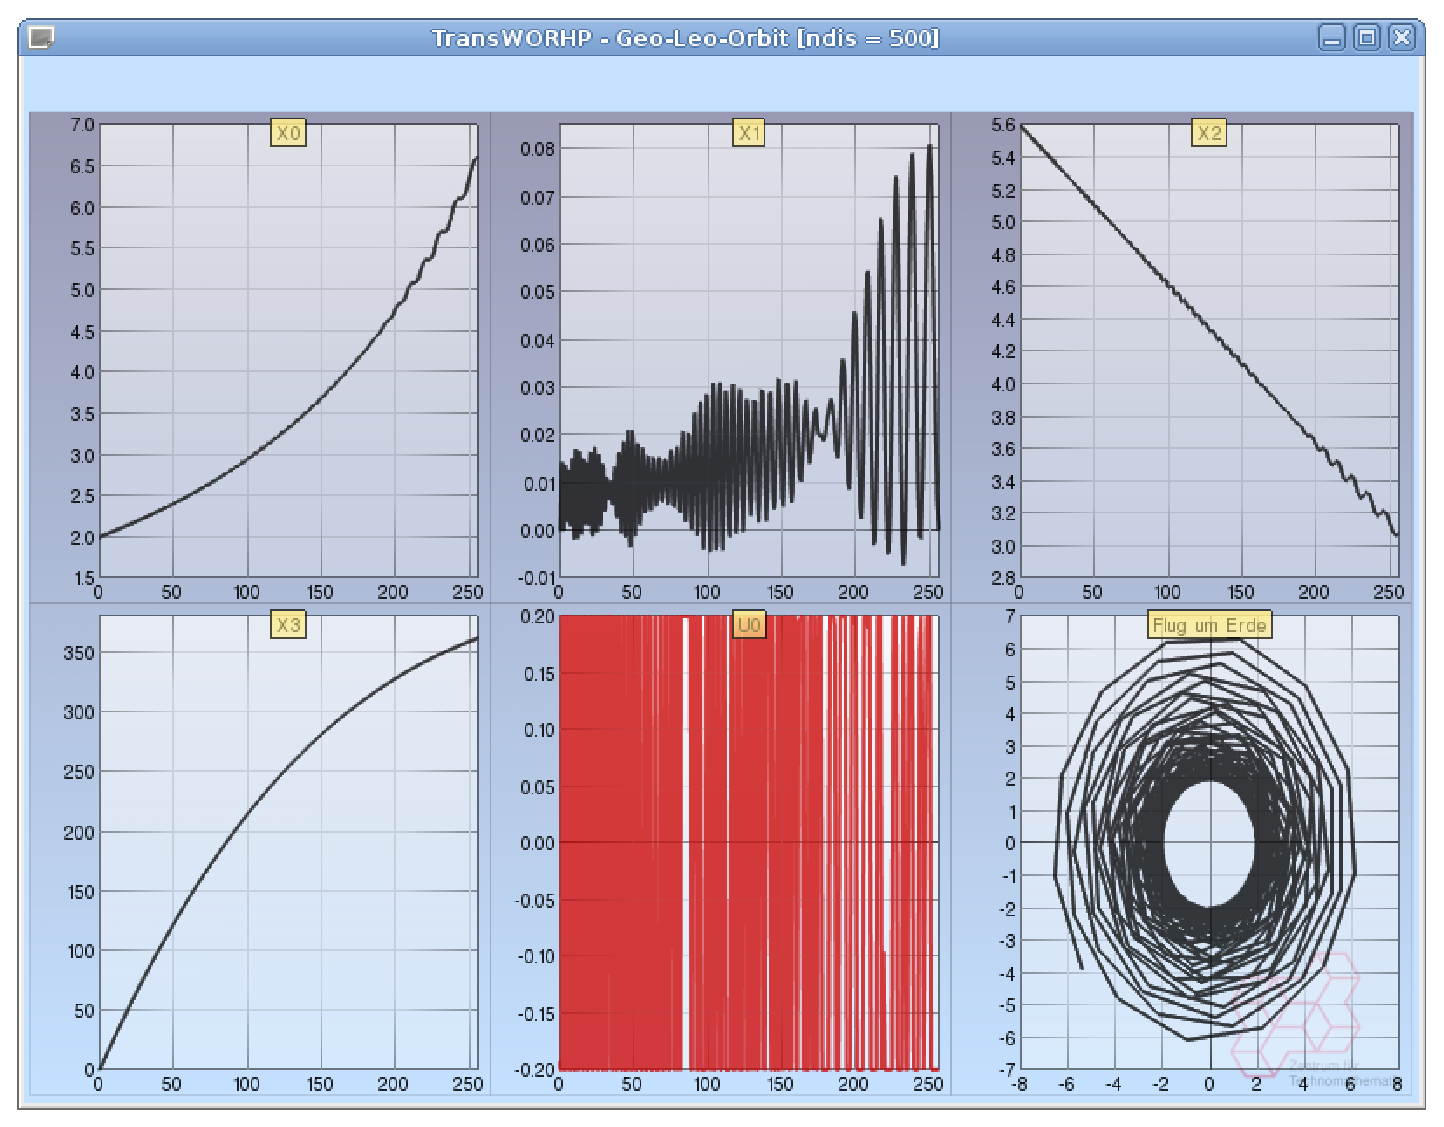
\includegraphics[width=10cm]{images/geoleo}
\caption{Phasenplot beim Geo-Leo-Transfer}
\label{abb2}
\end{center}
\end{figure}
